\chapter{Background}
In this chapter we provide a brief background on recommender systems and their growth over the years.


\section{Recommender Systems}
Recommender systems are essentially glorified information retrieval algorithms. They aim to predict a user's interest towards a web item by utilizing a variety of data ranging from the user's behaviour history to the actual content of the web item. Recommender systems have become a very popular phenomenon and are prevalent in the web, be it electronic retailers such as eBay and Amazon or social networking sites such as Facebook and Twitter, the underlying motivation across domains remains relatively the same - to retain the user on the site by delivering him content he would find interesting.

Earlier we discussed on how different forms of feedback affect recommendations. Now, we briefly discuss the major techniques employed in recommender systems.

\subsection{Collaborative Filtering}
\cite{goldberg_using_1992}
\begin{figure}[!h]
\centering
\begin{subfigure}[b]{0.4\textwidth}
    \centering
    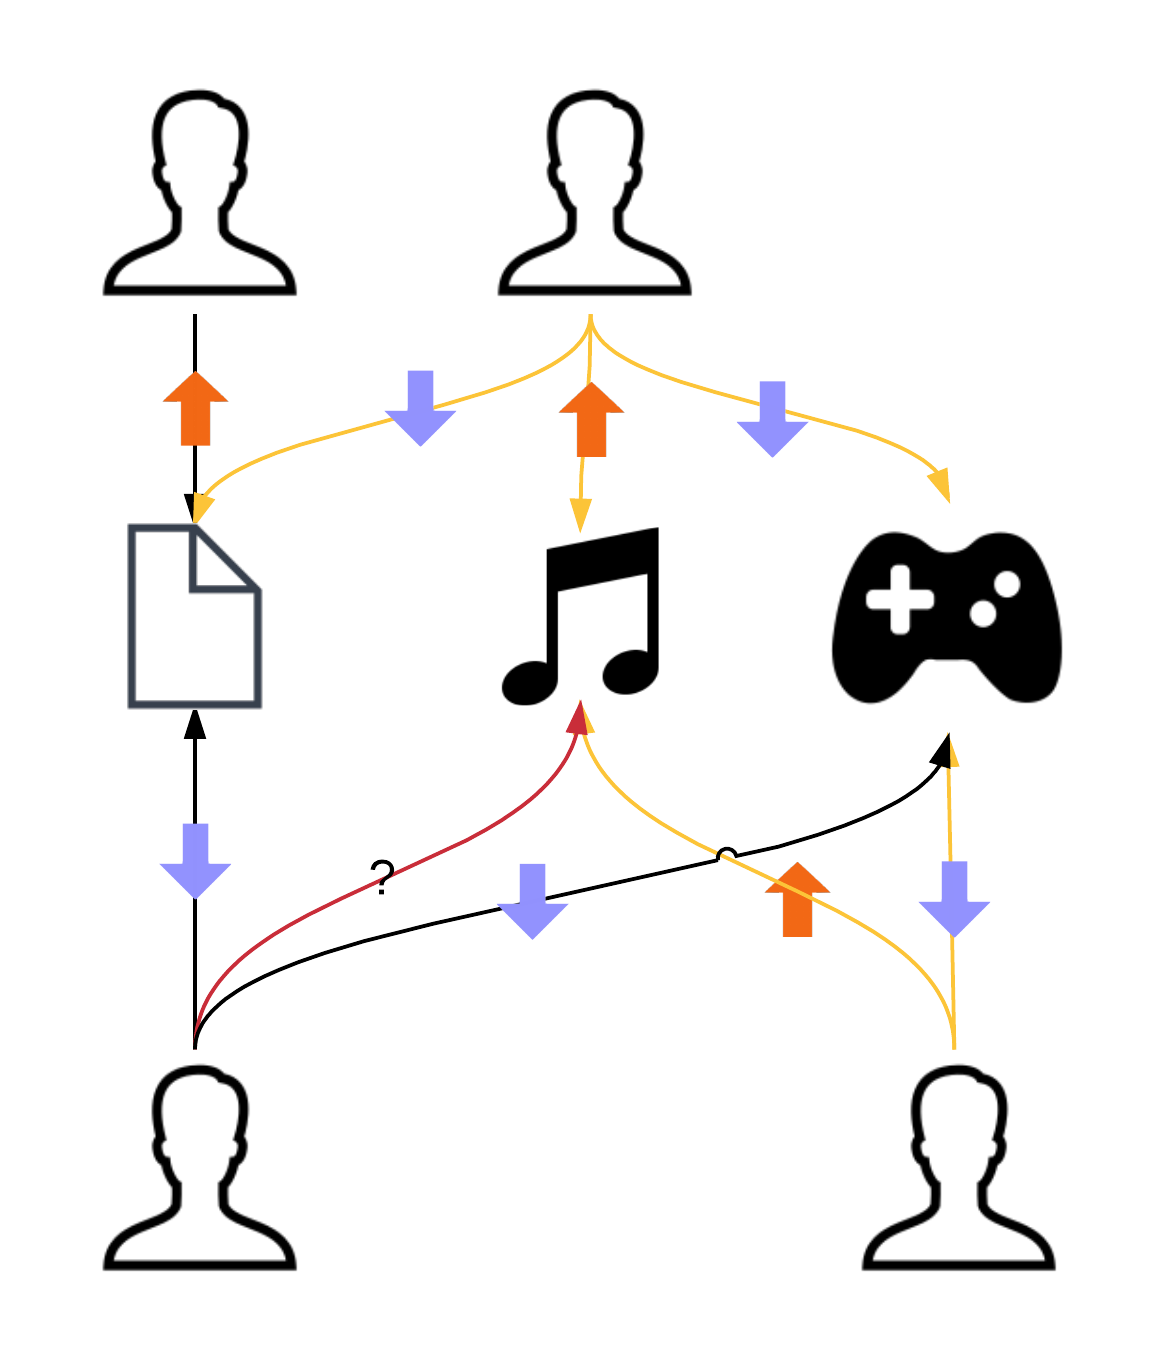
\includegraphics[width=\textwidth]{c-back_images/cf_1.png}
    \caption{Before Prediction}
    \label{fig:cf1}
\end{subfigure}
\hfill
\begin{subfigure}[b]{0.4\textwidth}
    \centering
    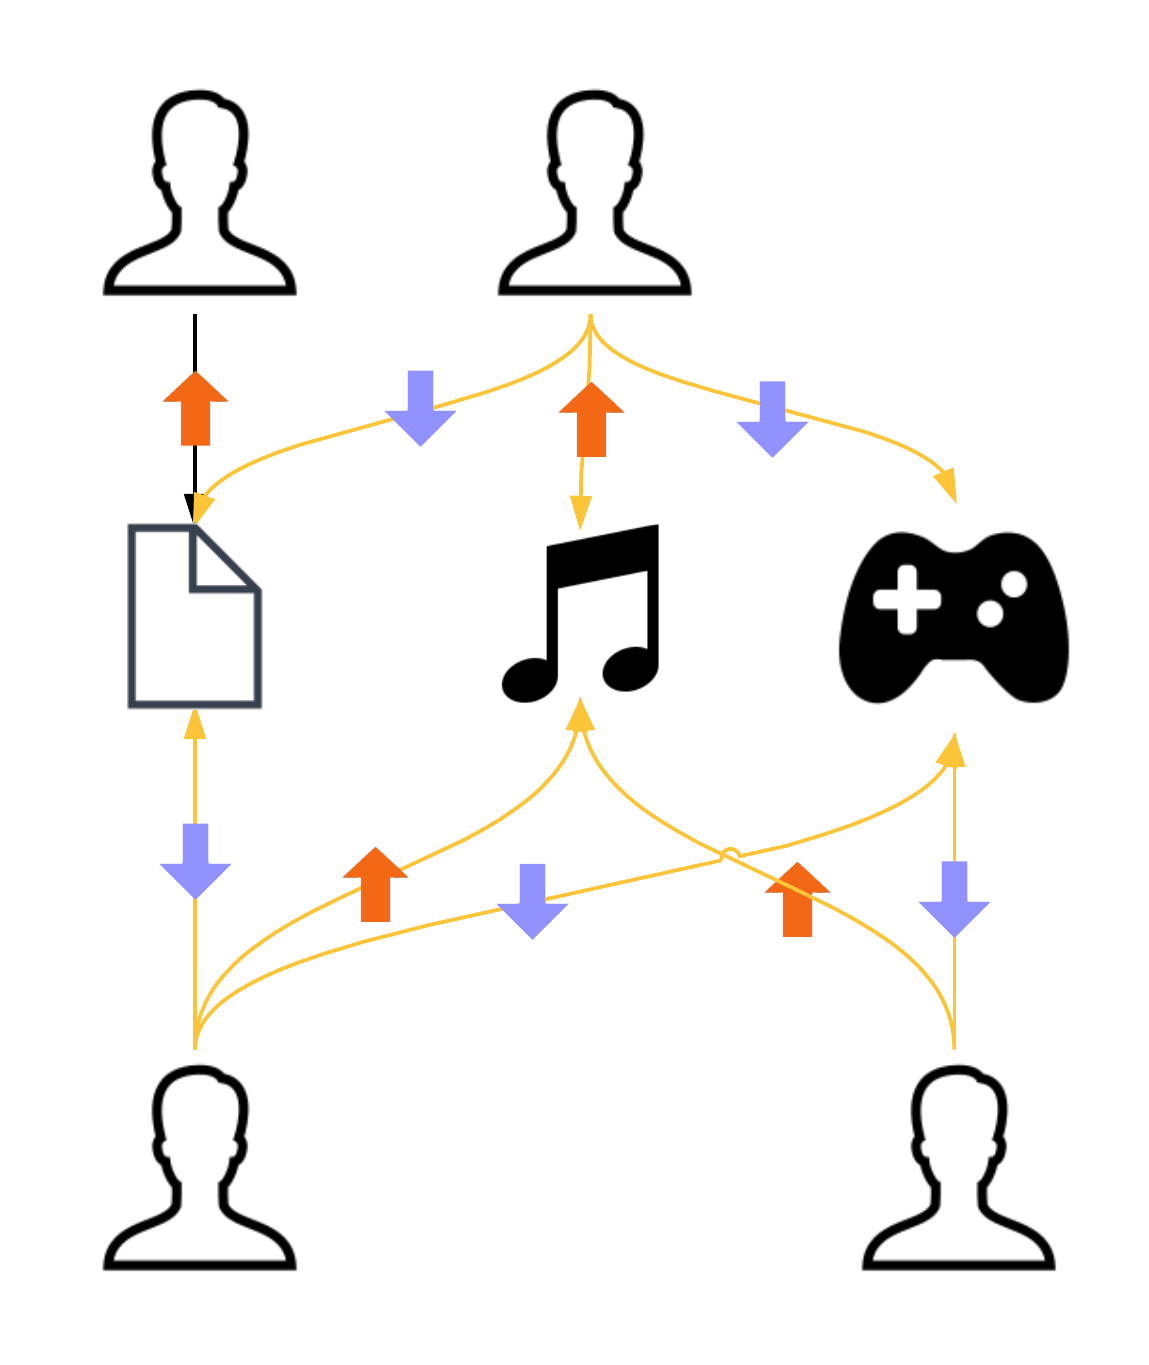
\includegraphics[width=\textwidth]{c-back_images/cf_2.png}
    \caption{After Prediction}
    \label{fig:cf2}
\end{subfigure}
\caption{Example of Collaborative Filtering}
\label{fig:cf}
\end{figure}

\subsection{Content Based Filtering}

\subsection{Hybrid Filtering}

The scope of this thesis lies in investigating the implications of comments and their content as a form of feedback.